\documentclass[aspectratio=169]{beamer}

% Input
\usepackage[utf8]{inputenc}
\usepackage[T1]{fontenc}
\usepackage{lmodern,charter}
\usepackage[letterspace=100]{microtype}
\usepackage{textcomp}
\usepackage{upquote}

% Beamer
\usepackage{beamercolorthemedove}
\usepackage{beamerinnerthemecircles}
\setbeamertemplate{navigation symbols}{}

% Tikz
\definecolor{burlywood}{cmyk}{1,1,1,1}
\usepackage{tikz}
\usetikzlibrary{arrows,calc,fit,positioning,shapes,chains}

% Graphics
\usepackage{graphicx}
\usepackage{epstopdf}
\DeclareGraphicsExtensions{.png,.pdf,.eps}

% Various
\usepackage[outline]{contour}
\contourlength{1.75pt}
\usepackage{enumitem}
\usepackage{hyperref}
\usepackage{minted}

% Title
\title{ZODB - the Python database}
\author{Asko Soukka <asko.soukka@iki.fi>}

% Begin
\begin{document}

\section{Title}

% Title
{
\usebackgroundtemplate{
\includegraphics[trim=0 0 0 0,clip,width=0.5\paperwidth]{images/asko.jpg}}
\begin{frame}[plain,t]
  \begin{columns}[onlytextwidth]
    \begin{column}{0.45\textwidth}
    \end{column}
    \begin{column}{0.45\textwidth}
      \vspace{0.5cm}
      \par
      \centering
      \href{http://iki.fi/asko.soukka/}{Asko Soukka},
      \href{mailto:asko.soukka@iki.fi}{asko.soukka@iki.fi}\\
      \href{https://github.com/datakure/}{github.com/datakurre}
      \vspace{0.5cm}
      \par
      \Huge
      \bfseries
      ZODB\\
      ---\\
      the Python database
      \par
      \large
      \mdseries
      \vspace{0.6cm}\par
      \href{https://www.jyu.fi/}{
\includegraphics[width=3.1cm]{images/logo.eps}}
    \end{column}
  \end{columns}
\end{frame}
}

% I give a small tutorial on getting started with ZODB with a simple command-line app written in Python 3. I cover the basic ZODB usage, testing and maintenance. Finally, I give a short overview of the ZODB ecosystem and demo of SubstanceD – a ZODB embracing web app framework.

{
\usebackgroundtemplate{
\includegraphics[trim=-100 0 0 -100,clip,width=0.5\paperwidth]{images/zodb.png}\hspace{1.92cm}\small PyCon Finland 31.10.2016}
\begin{frame}[plain,t]
  \begin{columns}[onlytextwidth]
    \begin{column}{0.45\textwidth}
    \end{column}
    \begin{column}{0.45\textwidth}
      \vspace{0.5cm}
      \par
      \centering
      ~\\~
      \vspace{0.5cm}
      \par
      \Huge
      \bfseries
      \href{http://zodb.org}{ZODB}\\
      ---\\
      the Python database
    \end{column}
  \end{columns}
\end{frame}
}

\section{Introduction}

%ZODB is a mature and well maintained object-oriented database for %ransparently and persistently storing Python object trees (objects and their references). In other words, ZODB stores Python objects as they are – no object-relational mapping required. In addition to Python objects, ZODB can also store binary blobs (like images) attached to those objects.

% https://www.youtube.com/watch?v=eGRJbBI_H2w
% http://www.substanced.net/

\begin{frame}[plain,t]
  \vspace{1.0cm}\par
  \Huge
  \bfseries
  \centering (Zope) Object Database
  \LARGE
  \vspace{1.0cm}\par
  \mdseries
  \begin{itemize}[label=--]
    \item Native object tree database for Python since 2002
    \item ACID transactions with snapshot isolation (MVCC)
%   \item FileStorage, BlobStorage, ZEO, ZRS
    \item ZODB, persistent, BTrees, transaction, zope.interface, ZConfig, zc.lockfile, zodbpickle (optional: ZEO, zc.zrs)
    \item Latest version: 5.0.0 (2016-09-06), Python 2.7, 3.4, 3.5
  \end{itemize}
\end{frame}

\section{Usage}

{
\usebackgroundtemplate{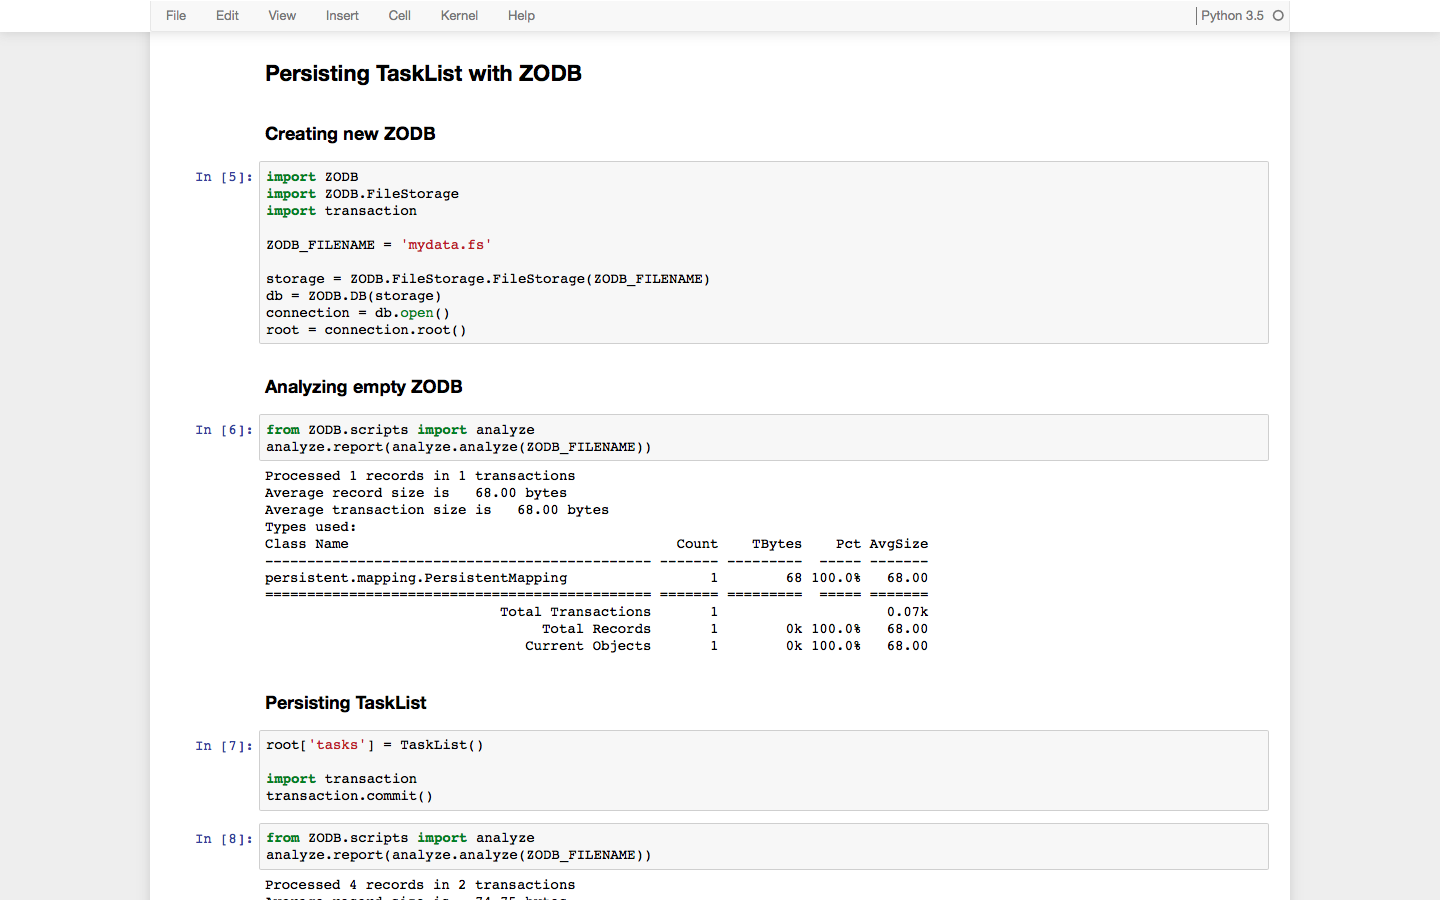
\includegraphics[trim=0 0 0 0,clip,width=\paperwidth]{images/jupyter.png}}%
\begin{frame}[plain,t]
  \setbeamercolor{background canvas}{bg=black}
  \vfill
  \centering
  \Huge
  \bfseries
  \lsstyle
  \contour{white}{Crash Course}
\end{frame}
}

\begin{frame}[plain,t]
  \vspace{1.0cm}\par
  \Huge
  \bfseries
  \centering ZODB can be a lot of fun
  \LARGE
  \vspace{1.0cm}\par
  \mdseries
  \begin{itemize}[label=--]
    \item It's implicit --- if object pickles, it persists.\\
    \normalsize
    Just remember to inherit your classes from Persistent.
    \LARGE
    \item It's pythonic and does object references right.
    \item It's safe, append only, immutable, but packs on request.
    \item It's fast, unless your code slows it down\ldots
%   \item Mutable objects should inherit their class from Persistent.
  \end{itemize}
\end{frame}

\section{Analysis}

\begin{frame}[plain,t]
  \vspace{1.0cm}\par
  \Huge
  \bfseries
  \centering Not necessarily \emph{web scale}
  \LARGE
  \vspace{1.0cm}\par
  \mdseries
  \begin{itemize}[label=--]
    \item Only one simultaneous request per connection.
    \begin{itemize}[label=\textbullet]
    \item Each connection has its own \emph{connection cache}.
    \item \emph{Connection cache} $=$ unpickled objects in RAM.
    \item Must be big enough to store the current working set.
    \end{itemize}
    \item Search indexes in ZODB are prone to write conflicts.
    \item No multi-master replication.
    \small But see
    \href{https://pypi.python.org/pypi/RelStorage}{RelStorage}
    and
    \href{https://pypi.python.org/pypi/neoppod}{neoppod}.
  \end{itemize}
\end{frame}

\begin{frame}[plain]
\begin{center}
\begin{tikzpicture}[
    start chain=going right,
    diagram item/.style={
        on chain
    }
]
\node[
    diagram item,
    label=center:Internet
]{\includegraphics{icons/cloud}};

\node[
    continue chain=going right,
    diagram item,
    join=with chain-1,
    label=below:Proxy
]{\includegraphics{"icons/3174 cluster contoller "}};

\node[
    continue chain=going right,
    diagram item,
    join=with chain-2,
    label=below:Httpd
]{\includegraphics{"icons/file server"}};

\node[
    continue chain=going above,
    diagram item,
    join=with chain-2,
    label=below:Httpd
]{\includegraphics{"icons/file server"}};

\node[
    continue chain=going right,
    diagram item,
    join=with chain-4,
    label=below:ZEO\,(ro)
]{\includegraphics{"icons/file server"}};

\node[
    continue chain=going above right,
    yshift=-1cm,
    diagram item,
    join=with chain-5,
    label=below:Storage
]{\includegraphics{"icons/relational database"}};

\node[
    continue chain=going below,
    diagram item,
    join=with chain-5,
    label=below:Storage
]{\includegraphics{"icons/relational database"}};

\node[
    continue chain=going below left,
    yshift=1cm,
    diagram item,
    join=with chain-5,
    label=right:ZRS
]{\includegraphics{icons/Services}};

\node[
    continue chain=going below right,
    yshift=1cm,
    diagram item,
    label=below:Storage
]{\includegraphics{"icons/relational database"}};

\node[
    continue chain=going below,
    diagram item,
    label=below:Storage
]{\includegraphics{"icons/relational database"}};

\node[
    continue chain=going above left,
    yshift=-1cm,
    diagram item,
    join=with chain-3,
    join=with chain-8,
    join=with chain-9,
    join=with chain-10,
    label=below:ZEO\,(rw)
]{\includegraphics{"icons/file server"}};


\node[
    continue chain=going left,
    diagram item,
    join=with chain-2,
    join=with chain-11,
    label=below:Httpd
]{\includegraphics{"icons/file server"}};

\end{tikzpicture}
\end{center}
\end{frame}

\section{Discussion}

{
\usebackgroundtemplate{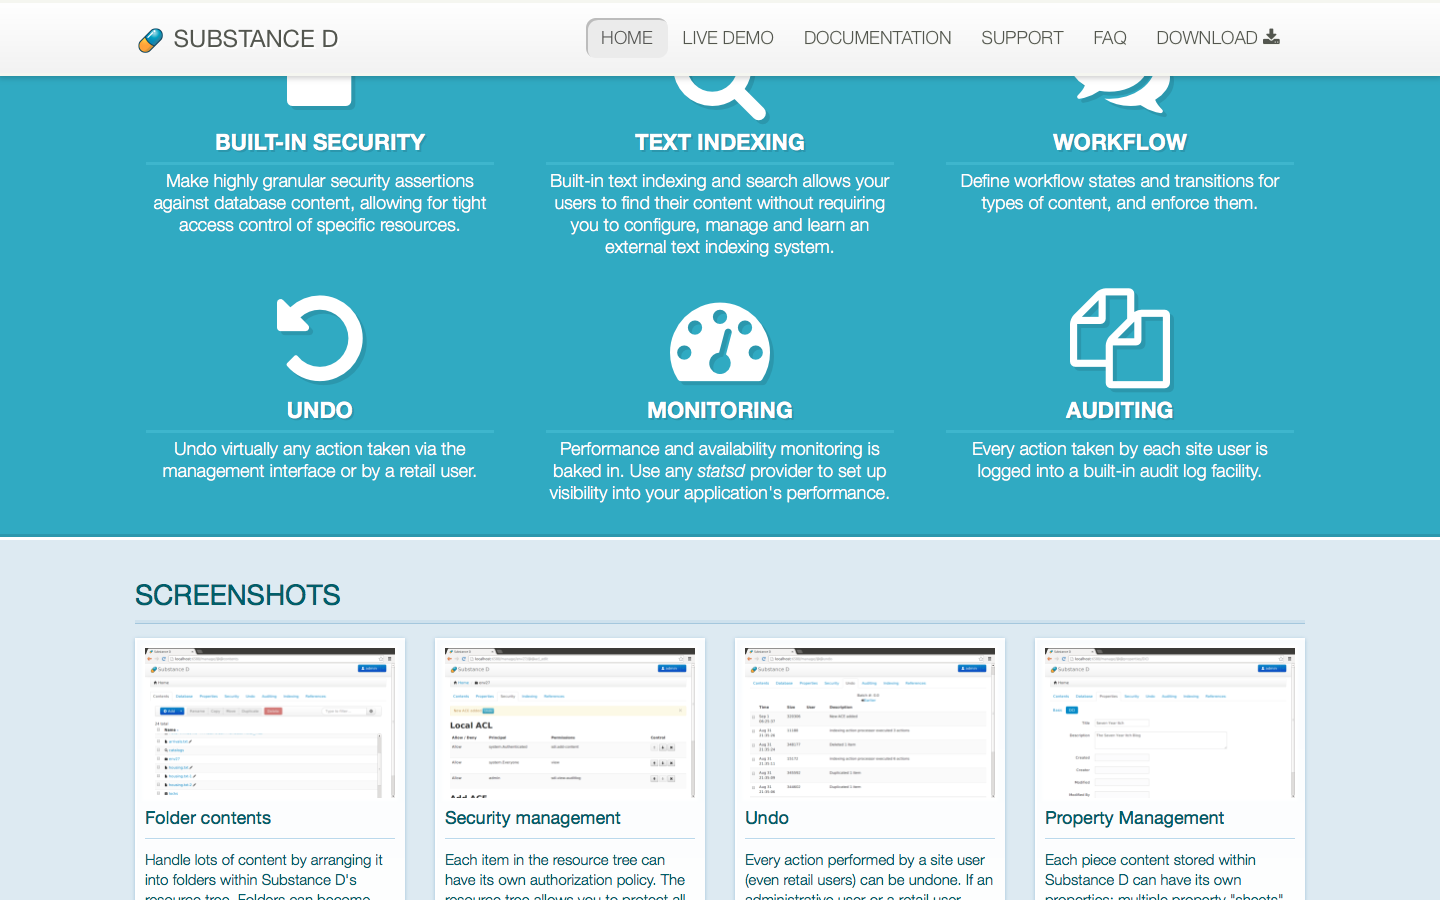
\includegraphics[trim=0 0 0 0,clip,width=\paperwidth]{images/substanced.png}}%
\begin{frame}[plain,t]
  \setbeamercolor{background canvas}{bg=black}
  \vfill
  \centering
  \Huge
  \bfseries
  \lsstyle
  \contour{white}{Substance D}
\end{frame}
}

\section{The End}

{
\usebackgroundtemplate{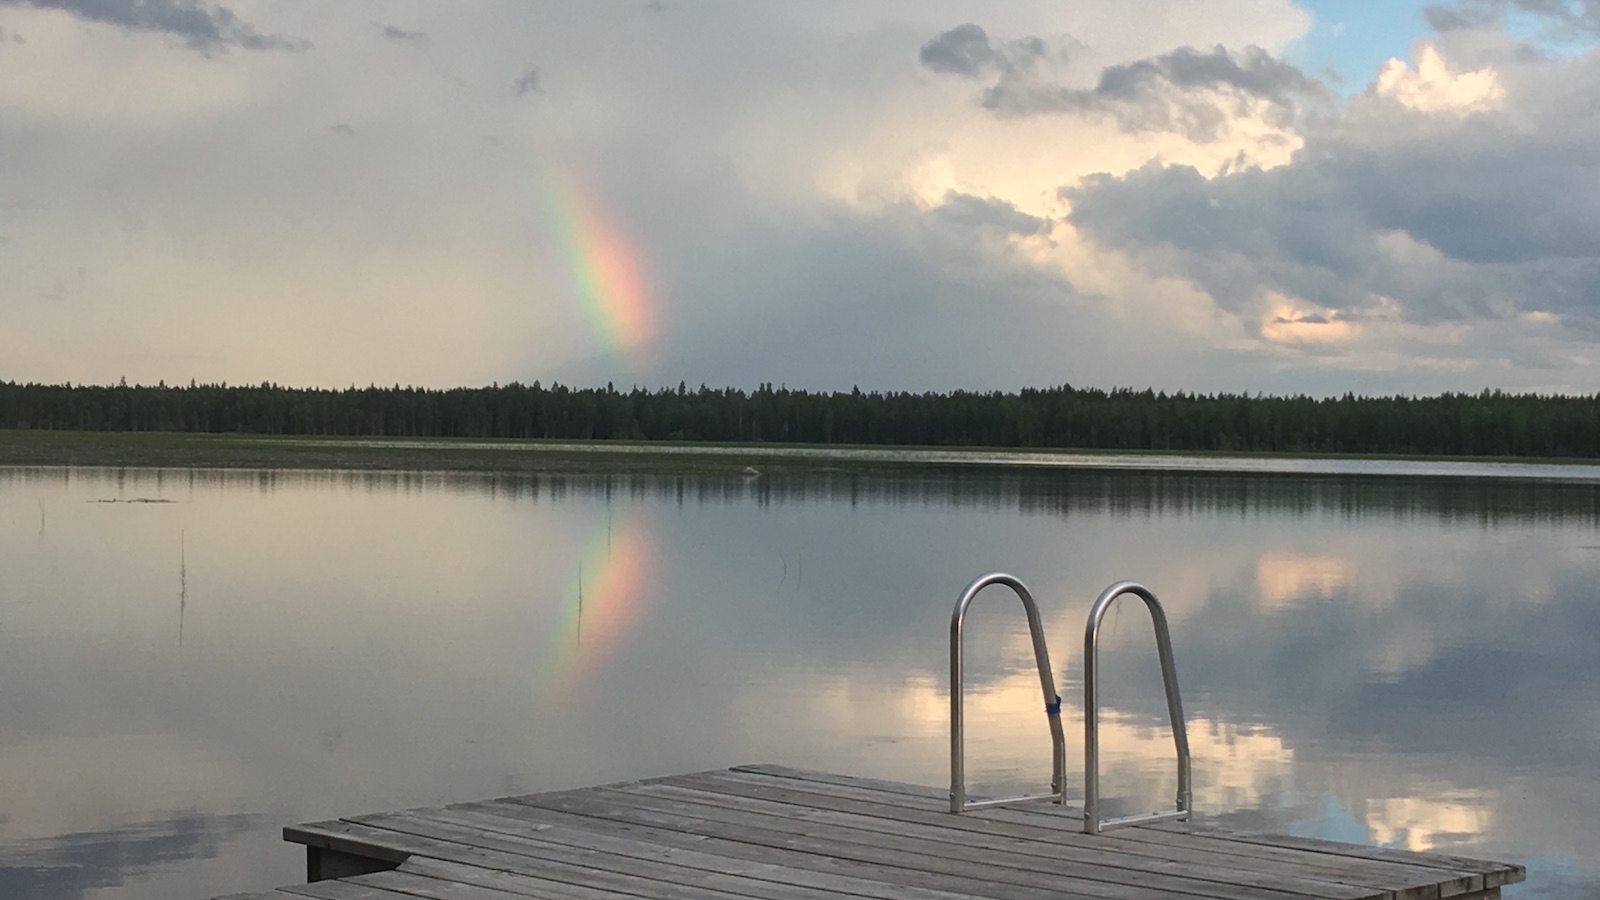
\includegraphics[trim=0 0 0 0,clip,width=\paperwidth]{images/questions.jpg}}%
\begin{frame}[plain,t]
  \setbeamercolor{background canvas}{bg=black}
  \vfill
  \centering
  \Huge
  \bfseries
  \lsstyle
  \contour{white}{Questions?}
  \par
  \large
  \contourlength{0.75pt}
  \contour{white}{github.com/datakurre/pyconfi2016}
\end{frame}
}

\end{document}
